%!TEX ROOT = ../centralized_vs_distributed.tex

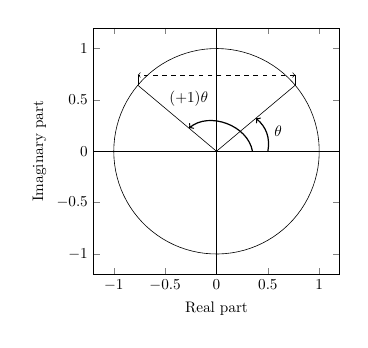
\begin{tikzpicture}[scale=.55]
	\begin{axis}[
		xlabel = Real part,
		ylabel = Imaginary part,
		axis equal image,
		ymin = -1.2,
		ymax = 1.2,
		xmin = -1.2,
		xmax = 1.2]
		\addplot [domain=-180:180, samples=100] ({cos(x)},{sin(x)});
		\draw (-1.2,0) -- (1.2,0);
		\draw (0,-1.2) -- (0,1.2);
		\draw (0,0) -- ({cos(40)},{sin(40)});
		\draw (0,0) -- ({-cos(40)},{sin(40)});
		\path[->,thick] (.5,0) edge[bend right] node [left] {}  ({.5*cos(40)},{.5*sin(40)});
		\path[->,thick] (.35,0) edge[bend right=60] node [left] {}  ({-.35*cos(40)},{.35*sin(40)}) ;
		\node at (.6,.2) {$ \delayn \theta $};
		\node at (-.27,.51) {$ (\delayn+1) \theta $};	
		\draw[<->,dashed] ({cos(40)},{sin(40)+.1}) -- ({-cos(40)},{sin(40)+.1});
		\draw ({cos(40)},{sin(40)+.1}) -- ({cos(40)},{sin(40)});
		\draw (-{cos(40)},{sin(40)+.1}) -- (-{cos(40)},{sin(40)});
		\node at (0.05,{sin(40)+.2}) {$ \gpos $};
	\end{axis}
\end{tikzpicture}